\section{Adaptive Open-Loop DPCM}
In this section we have to implement an a Differential Pulse Code Modulator. The functional scheme is presented on figure \ref{dpmc}.
\begin{figure}[!ht]
\centering
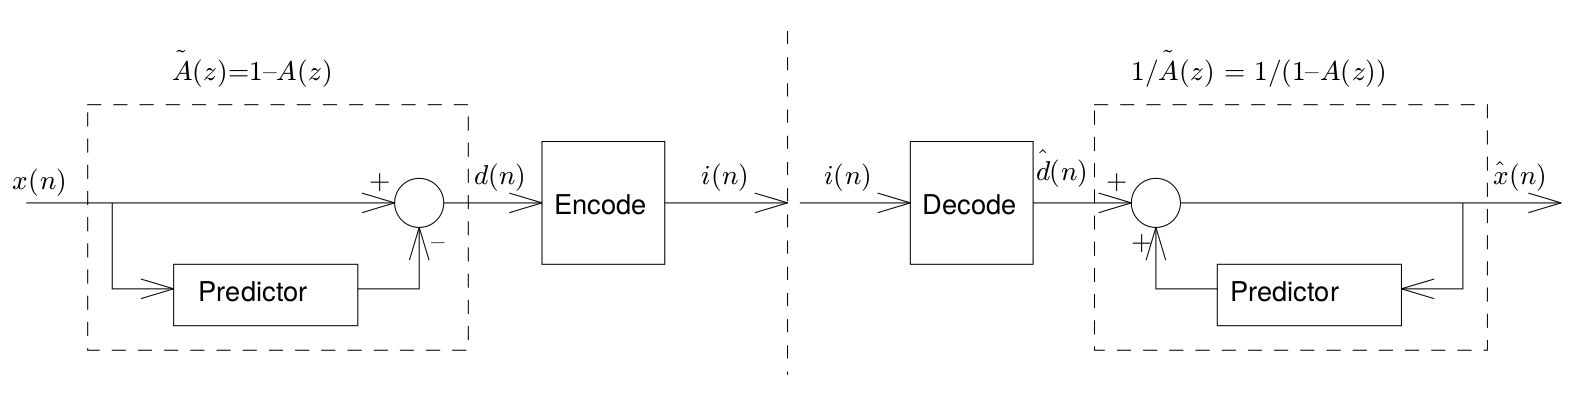
\includegraphics[scale=.3]{dpmc}
\caption{Functional scheme of a DPMC}
\label{dpmc}
\end{figure}

The idea here is to perform a linear prediction on an input signal, and to transmit the error signal with the prediction coefficient. It is not efficient to transmit a quantized input because the frames are strongly correlated between each other, as we can see on figure \ref{corr}.

\begin{figure}[!ht]
\centering
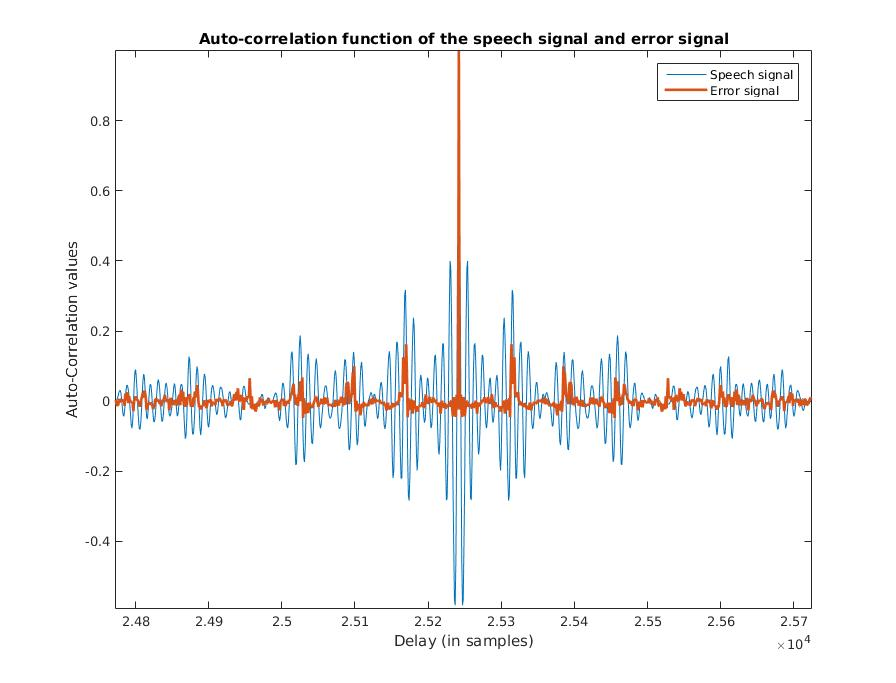
\includegraphics[scale=.4]{corr}
\caption{Correlation function of the input speech signal.}
\label{corr}
\end{figure}
%%% Local Variables:
%%% TeX-master: "master"
%%% End:

